% Apendice
\chapter{Informaci'on Adicional de SAP R/3}

	En este cap'itulo son presentadas algunas ilustraciones e informaci'on adicional donde se muestran algunos de los elementos presentes en el Cap'itulo~\ref{chap:ssimilar}.

\subsection{Estructura de una Empresa en el M'odulo SD de SAP}
Una empresa est'a conformada por un conjunto de unidades m'as peque\~nas que facilitan el trabajo en el proceso de ventas y sus actividades asociadas.
\newline
Las unidades m'as importantes que componen a una empresa correspondientes al 'area de Ventas y Distribuci'on son las que se listan a continuaci'on:

\begin{itemize}
\item Organizaci'on(es) de Ventas
\item Canal(es) de Distribuci'on
\item Sector(es)
\item 'Areas de Ventas
\item Oficinas de Venta
\item Puestos de Expedici'on
\item Puestos de Carga
\end{itemize}

	En los pr'oximos puntos se ahondar'a mas en cada una de estas unidades, para as'i conocer en detalle en qu'e consiste cada una.
	
\subsubsection{Organizaci'on de Venta}
	Una \textbf{Organizaci'on de Venta} dentro del Sistema SAP es una unidad que es muy utilizada para poder dar a conocer y distribuir los bienes y servicios que la empresa ofrece. A trav'es de esta unidad, se pueden realizar las distintas negociaciones emtre el cliente y la empresa, asi como los t'erminos y condiciones a los que llegan ambos, como por ejemplo el establecimiento de alg'un tipo de descuento, la forma de pago (si es de contado, en 15 d'ias, etc). 
	
\subsubsection{Canal de Distribuci'on}
	Un \textbf{Canal de Distribuci'on} dentro de SAP es una unidad que es capaz de distribuir los bienes y servicios que son ofrecidos por la Organizaci'on de Ventas a los clientes que atiende.
	Para poder llevar esta tarea a cabo, es posible que sea necesario usar m'as de un canal de distribuci'on. Es por ello que una Organizaci'on de Ventas tiene a su cargo almenos un Centro de Distribuci'on, aunque pudieran ser varios, dependiendo ya del proceso que lleve la empresa en particular.

\subsubsection{Sector}
	Un \textbf{Sector (o Divisi'on por su nombre en ingl'es)} dentro de SAP es una unidad organizativa que permite agrupar cada uno de los productos o materiales que son ofrecidos por las Organizaciones de Ventas en diferentes categor'ias. 
	
\subsubsection{'Area de Ventas}
	Un \textbf{'Area de Ventas} es una relaci'on existente entre una Organizaci'on de Ventas, un Canal de Distribuci'on y un Sector. Todas las transacciones relacionadas con Ventas y Distribuci'on son manejadas a trav'es de las 'Areas de Ventas.
	
\subsubsection{Oficina de Ventas}
	Una \textbf{Oficina de Ventas} es el lugar f'isico donde la empresa realiza la venta de bienes y servicios. Es importante resaltar que estas unidades pueden estar ubicadas en distintos puntos geogr'aficos. 
	Un 'Area de Ventas tiene asociada a almenos una Oficina de Ventas, aunque puede tener varias bajo su cargo.

\subsubsection{Puestos de Expedici'on}
	Un \textbf{Puesto de Expedici'on} es el lugar f'isico que posee la empresa para efectuar las entregas de los bienes producidos y adquiridos.
	Un puesto de expedici'on puede estar asociado a un Centro, pero no es limitativo. Es decir, que puede estar asociado a varios Centros.
	Algo importante que resaltar es que para que una entrega se pueda efectuar dentro de SAP, es necesario indicar en cu'al Puesto de Expedici'on se desea hacer, ya que de lo contrario, no es posible.
	
\subsubsection{Puestos de Carga}
	Un \textbf{Puesto de Carga} es una sub-divisi'on de los Puestos de Expedici'on. 

\section{Componentes de un Programa en ABAP/4}{sect:proabap}
\subsubsection*{DECLARACI'ON DE DATOS GLOBALES, CLASES Y SELECTION SCREENS (PANTALLAS DE SELECCION)}
	En esta parte es donde se llevan a cabo las declaraciones de los datos globales, de las pantallas de selecci'on y de las clases. A continuaci'on, se proceder'a a explicar cada uno de estos puntos.
\subsubsection*{Datos Globales}
	Los Datos Globales es el conjunto de datos que son declarados con el fin de poder acceder a ellos y poder utilizarlos a lo largo del programa. Estos datos globales constan de:
\begin{itemize}
\item Variables
\item Constantes
\item Estructuras de Datos
\item Tablas Internas
\end{itemize}

\subsubsection*{Clases}
	Una clase en SAP es conocida como una plantilla para un objeto. Tambi'en se puede definir como una descripci'on abstracta de un objeto.

\subsubsection*{Selection Screens (Pantallas de Selecci'on)}
	Las Pantallas de Selecci'on son unas pantallas especiales que son definidas en ABAP/4 para permitir que los programas reciban datos provenientes de los usuarios a trav'es de la entrada est'andar (Teclado). El ambiente de ejecuci'on de ABAP controla el flujo del procesamiento de las pantallas de selecci'on. De esta manera, este ambiente genera un n'umero de eventos antes de que las pantallas de selecci'on sean mostradas, y otros luego despu'es que las mismas hayan sido ejecutadas.
	
\subsubsection*{CONTENEDOR DE BLOQUES DE PROCESAMIENTO}
	Esta segunda parte est'a compuesta por los Bloques de Procesamiento, entre los cuales se pueden encontrar los que se listan a continuaci'on:
\begin{itemize}
\item M'odulos de Di'alogo
\item Bloques de Eventos
\item Procedimientos (m'etodos, subrutinas y m'odulo de funciones con sus datos locales)
\end{itemize}

\subsubsection*{BLOQUE DE PROGRAMA}
	Consiste en todos los estados ABAP (salvo estados declarativos, los cuales van en la primera parte).
	
\subsubsection*{BLOQUE DE PROCESO DE LLAMADAS}
	En esta tercera parte es posible hacer llamadas a otros bloques externos o internos al programa ABAP. Los m'odulos de Di'alogo y los bloques de eventos son llamados desde afuera. Los procedimientos son llamados usando instrucciones ABAP. 
	
\section{Componentes de un Smartform}
\subsubsection{Constructor de Formularios Inteligentes (Smart Form Builder)}
	Esta componente es la interfaz principal que es usada para la construcci'on de Smartforms a trav'es de la pantalla inicial que se muestra en la Figura ~\ref{fig:smartforms1}, en donde a trav'es de esta transacci'on es posible crear, modificar o visualizar un smartform. Al darle click a cualquier opci'on, la misma lleva a otra pantalla, la cual es la que permite la construcci'on de un smartform. 'Esta es conocida como \textbf{Smart Form Builder}. En la Figura ~\ref{fig:builder} en donde es posible visualizar varias partes bien diferenciadas, las cuales se explican a continuaci'on:
\begin{itemize}
\item Men'u de Navegaci'on: Es el que est'a representado por la columna izquierda. 'Este expone al formulario en forma de jerarqu'ia, dode cada elemento es un nodo
\item Marco de Mantenimiento: Est'a conformado por los atributos principales del formulario (Nombre y significado)
\item Lista de Campos: Esta lista muestra los datos que est'an definidos actualmente en el formulario
\item Form Painter: 'Esta es una herramienta gr'afica la cual permite dise\~nar cada una de las partes que tendr'a el formulario.
\end{itemize}
\subsubsection{Template de impresi'on para el Smartform (Smart Form Print Form Template}
	Un template de impresi'on para el Smartform ofrece un dise\~no ya creado por el sistema para as'i crear un Smartform que pueda ser imprimible.
\subsubsection{M'odulo de Funciones del Smart Form (Smart Form Function Module)}
	El M'odulo de Funciones del Smart Form es una secuencia de instrucciones generadas de forma autom'atica al momento de la activaci'on del  mismo.
\subsubsection{Programa de Impresi'on de Smart Forms (Smart Form Print Program)}
	El Programa de Impresi'on de Smartforms es el programa control encargado de manejar la informaci'on que es enviada al smartform y de su posterior impresi'on. 
\section{Etapas pertenecientes a la Fase de la Realizaci'on de ASAP}{sect:realizacion}
\subsubsection{Simulaci'on}
	El primer paso que se lleva en esta etapa es la configuraci'on. Aqu'i, los distintos consultores configuran el sistema SAP de acuerdo al documento del Negocio previamente definido.  Esta configuraci'on cubre el 80 de los procesos del negocio de la compa\~n'ia y de las transacciones diarias. Este proceso implica modificar el software de SAP a trav'es de procedimientos no programables, como por ejemplo:  modificaciones de entrada a tabla, herramientas base, etc.
	El siguiente paso dentro de esta etapa es la Reproducci'on. 'Este consiste en introducir un conjunto reducido de usuarios en el nuevo sistema para hacer las pruebas a la configuraci'on realizada previamente, y as'i poder obtener una retroalimentaci'on. Las reproducciones son realizadas de forma peri'odica bas'andose en las preferencias de los usuarios. 
	
\subsubsection{Validaci'on}
	Durante esta etapa, el dise\~no es refinado y finalizado. El equipo de trabajo refina el sistema de tal modo que todos los requerimientos del negocio se encuentren configurados. 
	Un punto importante durante la realizaci'on de esta fase es la elaboraci'on de una lista de procesos maestros. 	El equipo involucrado comienza a desarrollar los procedimientos del procedimiento del Negocio (Gu'ia de Configuraci'on), con la cual se documenta toda la configuraci'on realizada al sistema. 
\subsubsection{Uni'on y Pruebas de Integraci'on}
	Para que un software sea colocado en producci'on debe haber recibido todas las pruebas necesarias. Un software que no es probado de la manera adecuada, puede traer consecuencias a la hora de ponerse en reproducci'on, como por ejemplo que se presente alguna falla inesperada, lo que derivar'ia en descartar el programa.
	El hecho de realizar una prueba a un sistema ERP integrado representa un gran desaf'io, pero dentro de los beneficios a obtener est'an los siguientes: 
\begin{itemize}
\item Se confirma que el proceso trabaja adecuadamente
\item Se obtiene una configuraci'on 'agil
\item Tiene rendimiento garantizado
\item La integraci'on es mejorada
\item Sus costos son bajos
\item Los riesgos se reducen al m'inimo
\end{itemize}
Las pruebas de todo el sistema implementado se realiza en dos grandes grupos: El primer grupo es el conjunto de pruebas unitarias. Estas consisten en realizar pruebas a peque\~nas transacciones, como por ejemplo: crear una orden de venta, crear un cliente, etc. Para esto, se hace por cada 'area funcional o m'odulo cumpliendo un ciclo b'asico, como por ejemplo, en Ventas y Distribuci'on el ciclo b'asico consiste en: Realizar el pedido de Venta, luego efectuar la entrega para as'i finalmente generar la factura correspondiente. 
El segundo grupo de pruebas est'a conformado por las \textbf{Pruebas Integrales}. 'Estas consisten en crear un conjunto de escenarios que involucren todas las 'areas funcionales implementadas. Estas pruebas son dise\~nadas con una perspectiva orientada a procesos. Por ejemplo, se prueba cada paso requerido para realizar un Pedido de Venta. En este punto, es fundamental contar con la presencia de los usuarios finales, ya que son ellos los que pueden brindar una retroalimentaci'on oportuna, y as'i poder detectar posibles fallas.
	Existen dos maneras de aplicar estas pruebas unitarias. La primera, se conoce como \textbf{Aseguramiento de Calidad (QA por su nombre en ingl'es)}, es realizada por un conjunto de miembros de tiempo completo en compa\~n'ia de usuarios del negocio pertenecientes a las distintas 'areas funcionales. Cada grupo es asignado a un peque\~no escenario, y es responsable de verificar que todo el proceso involucrado se lleve a cabo sin errores desde el inicio hasta el final. La segunda opci'on es tener distintos grupos que realizen las distintas pruebas por cada 'area funcional. En el caso de que la prueba involucre varias 'areas funcionales, por ejemplo, se tienen las 'areas funcionales A, B y C. En el momento en que el 'area A necesite enviar recursos al 'area B, la responsabilidad de las pruebas pasa del miembro del equipo A que est'a ejecutando la prueba, a alg'un miembro del equipo B.

\subsubsection{Conversi'on y Carga de los Datos}
	Para que el sistema implementado en SAP pueda funcionar correctamente, es necesario realizar la carga de una gran cantidad de datos. 
	Existen dos m'etodos para la migraci'on de los datos dentro del sistema SAP, estos son los que se listan a continuaci'on:
\begin{itemize}
\item Entrada por Lote: Consiste en simular la entrada de datos a trav'es de las pantallas de las distintas transacciones.
\item Entrada Directa: Se recibe el archivo de forma directa, se procesa, se realizan los chequeos previos a los datos, y luego se realiza la actualizaci'on en la Base de Datos.
\end{itemize}
	Es importante que la migraci'on de los datos se realice lo m'as temprano posible. Se recomienda agrupar los datos en peque\~nos grupos, e ir carg'andolos poco a poco. Sin embargo, esto deriva en una limitaci'on de la efectividad a la hora de continuar con las configuraciones, dado que el sistema se encuentra incompleto y puede presentar fallas a la hora de la carga de estos datos.
	En SAP, los datos se pueden agrupar en 5 grupos principales:
\begin{itemize}
\item Datos Maestros Automatizados
\item Datos Maestros Manuales
\item Datos de Transacci'on Automatizados
\item Datos de Transacci'on Manuales
\item Datos de Limpieza
\end{itemize}
	Existe un problema muy importante que hay que tomar en cuenta, y que por lo general se ignora o no se le da la debida importancia: El problema de los datos sucios o inconsistentes. Esto es fundamental, ya que pueden generar prblemas con el sistema implementado en SAP por la calidad de los datos que han sido cargados. 
	Otro problema con el que se debe estar alerta es con la duplicidad de los datos, ya que por ejemplo, se puede tener un material con m'ultiples entradas. Esto se debe a que dentro de la entrada de un material, el 'unico campo un'ivoco correspondiente a dicho material es un c'odigo asignado por SAP. 
	Existen dos maneras de chequear que los datos no tengan duplicados: La primera, se realiza en el sistema original de donde provienen los datos. La segunda, se realiza una vez que los datos hayan sido ingresados a SAP, se procede a su chequeo correspondiente.
	Las personas encargadas del chequeo de los datos son los usuarios finales, ya que, son ellos quienes conocen dichos datos y pueden ser capaces de descartar cualquier inconsistencia que pueda ser encontrada.

\subsubsection{Interfaces, Ampliaciones y Reportes}

	Para poder asegurar aquellos peque\~nos sub-sistemas que se pierden del sistema original a la hora de adaptar el negocio de una empresa en SAP, es necesario la creaci'on de interfaces. Las interfaces en SAP se encargan de ayudar en la integraci'on del proceso del negocio y la sincronizaci'on de los datos entre dos o m'as sistemas SAP, o entre SAP y un sistema externo.
	Adicionalmente, para poder adaptar las implementaciones realizadas a las necesidades espec'ificas de la empresa, es posible que sea necesario la creaci'on de una \textbf{Ampliaci'on}. Una Ampliaci'on b'asicamente es una modificaci'on peque\~na que se les puede aplicar a programas est'andares ya existentes dentro del Sistema SAP. Para esto, es necesario que dentro del equipo del proyecto, existan personas que sepan programar en ABAP, ya que dichas ampliaciones son realizadas en este lenguaje. El problema con esto, es que necesita ser probado constantemente, sobre todo cuando existan actualizaciones al software de SAP. 
	Otra herramienta que suele ser importante durante esta fase son los reportes realizados, ya que hay muchas cosas que quiz'as la empresa necesite, que con las transacciones existentes no se pueden realizar.
	Los requerimientos para realizar dichos reportes deben ser establecidos lo m'as temprano posible, para que as'i puedan ser agrupados de acuerdo a la prioridad que tenga dicho requerimiento. Para la realizaci'on de dichos requerimientos, es necesario contar con el grupo de programadores en ABAP. 
	
	
\section{Figuras Adicionales de SAP}
\begin{figure}[H]
\centering
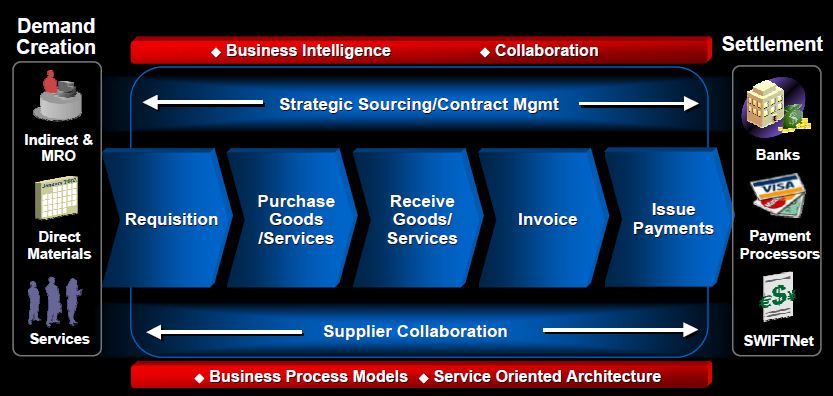
\includegraphics[scale=1.0,type=jpg,ext=.jpg,read=.jpg]{figures/salesFlow}
\caption{Proceso de Ventas y Distribuci'on en SAP}
\label{fig:salesFlow}
\end{figure}

\begin{figure}[htb]
\centering
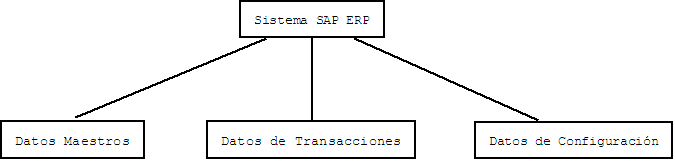
\includegraphics[scale=0.45,type=png,ext=.png,read=.png]{figures/Clasificacion1}
\caption{Clasificaci'on de los datos en el M'odulo SD}
\label{fig:datasd}
\end{figure}

\section{Im'agenes Adicionales de ABAP/4}
\begin{figure}[H]
\centering
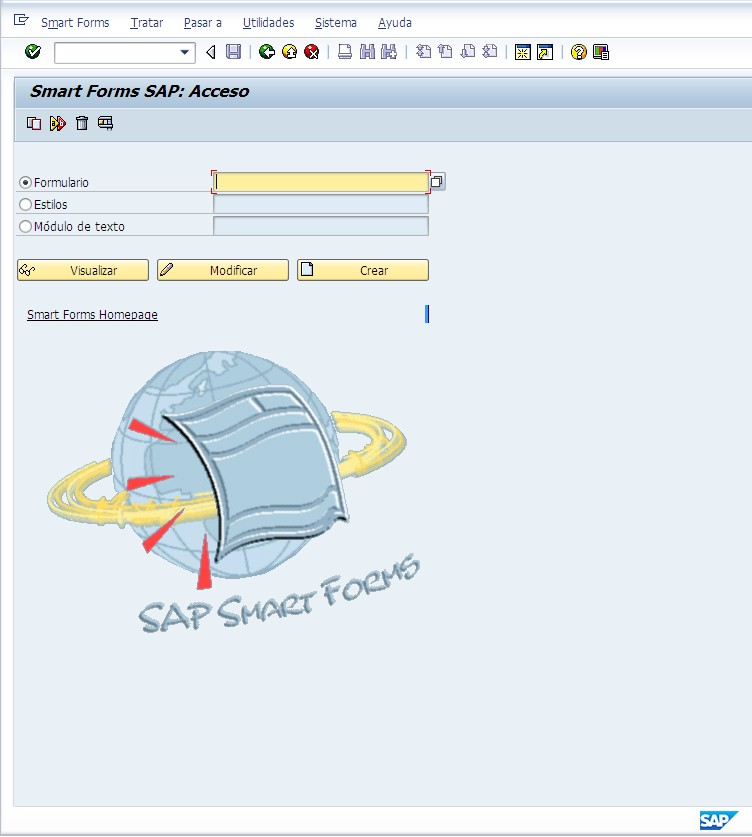
\includegraphics[scale=0.65,type=jpg,ext=.jpg,read=.jpg]{figures/sm_initial}
\caption{Pantalla Inicial de la transacci'on SMARTFORMS}
\label{fig:smartforms1}
\end{figure}

\begin{figure}[H]
\centering
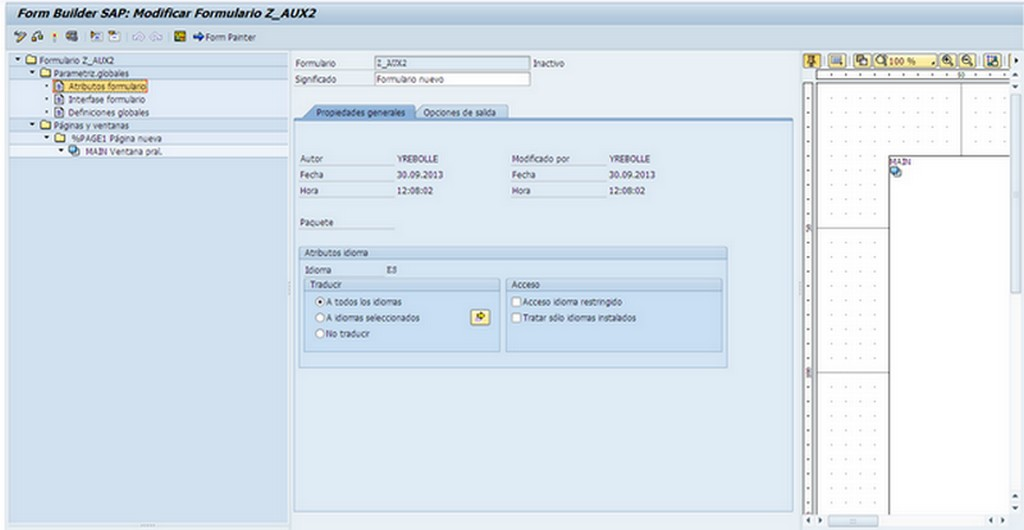
\includegraphics[scale=0.65,type=jpg,ext=.jpg,read=.jpg]{figures/builder}
\caption{Smart Form Builder}
\label{fig:builder}
\end{figure}

\begin{figure}[H]
\centering
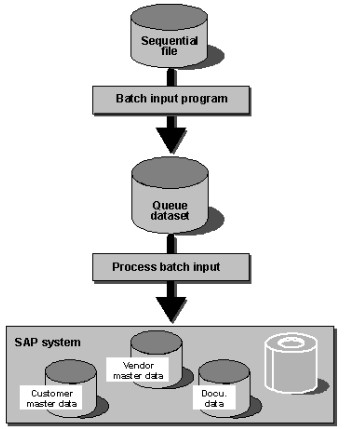
\includegraphics[scale=1.0,type=jpg,ext=.jpg,read=.jpg]{figures/batch_input_process}
\caption{Proceso de Batch Input ejecutado en SAP}
\label{fig:process}
\end{figure}

\section{Im'agenes Adicionales de la Metodolog'ia ASAP}
\begin{figure}[htb]
\centering
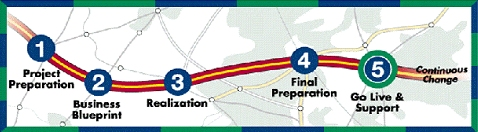
\includegraphics[scale=0.65,type=jpg,ext=.jpg,read=.jpg]{figures/roadmap}
\caption{Mapa de Rutas usado en ASAP}
\label{fig:roadmap}
\end{figure}